%	Proposta projeto de API  
%	Jean Henrique Ferreira Freire 
%

 \documentclass{abnt}
 \usepackage[brazil]{babel}
 \usepackage[utf8]{inputenc}
 \usepackage[num]{abntcite}
 \usepackage{comment}
 \usepackage{cite}
 \usepackage{graphicx}
 \usepackage{amsmath,amsfonts}
 \usepackage{subfigure}
 \usepackage{comment}
 \usepackage{times,amsmath,epsfig}
 \usepackage{graphicx,url}


\begin{document}

\autor{Jean Henrique Ferreira Freire\\Lucas Antonio Conceição de Castro}

\titulo{Proposta Trabalho Pratico Sistemas de Tempo Real:\\ Robôs Autônomos de
busca}

\instituicao{Universidade Federal de Minas Gerais \par Instituto de Ciências Exatas \par Departamento de Ciência da Computação}

\local{Belo Horizonte} \data{2013}

\folhaderosto

\begin{resumo}
    Um sistema de tempo real, é um sistema que possui conjunto de tarefas que
    devem ser executadas em um intervalo de tempo pre determinado. Uma das
    aplicações deste tipo de sistema e a robótica, neste
    trabalho propomos um sistema de tempo real para controlar, inicialmente,
    dois robôs autônomos de busca. Modelamos o sistema utilizando os conceitos
    de sistemas de tempo real, e apresentamos um cronograma com etapas e prazos
    para concluir o projeto.
\end{resumo}

\chapter{Introdução} \label{intro}


    Em sistemas operacionais padrões, como o Windows e o Linux por exemplo, um
    programa qualquer e executado em um certo intervalo de tempo e quanto menor for
    esse intervalo melhor é a performance do sistema, porem não existem restrições
    quanto ao valor desta variável. Em um sistema de tempo real cada programa tem um
    tempo máximo para ser executado(deadline), e sua execução depois deste
    tempo não só é indesejada como em muitos casos e inútil, deste modo, em
    sistemas de tempo real o tempo de execução deixa de ser um fator de
    performance pra se tornar um fator critico.

    Uma das muitas aplicações de um sistema de tempo real e a robótica, neste
    tipo de sistema os robôs devem interagir com o ambiente e tomar decisões
    baseadas nos resultados dessa interação, eles podem ser caracterizados como
    um sistema de tempo real pois, em geral, o tempo de resposta a estes
    estímulos do ambiente deve ser feito em um curto espaço de tempo ou as
    condições do ambiente se alterem.

    Neste trabalho nos propomos um sistema de tempo real que vai controlar
    dois robôs de busca concorrentes, estes robôs vão se comunicar com servidor
    central que vai transmitir os pontos de busca, cada robô deve calcular um
    caminho ate o ponto que julga ter capacidade de chegar primeiro, logo em
    seguida deve caminhar até este ponto enviando ao servidor periodicamente
    sua posição, e enviando uma mensagem de sucesso a cada ponto alcançado. Por
    sua vez o servidor fica a cargo de atualizar a lista de pontos disponíveis
    quando necessário alem de informar a cada carro a posição dos outros a fim
    de evitar colisões.

    Apresentamos também  as especificações de hardware, e o protocolo
    de comunicação que já vem sendo implementado.
     
    O restante deste relatório esta organizado da seguinte forma, o capítulo
    ~\ref{objt} apresenta os objetivos do trabalho, o capítulo ~\ref{metod}
    apresenta a metodologia abordada, o capítulo ~\ref{result} lista os
    resultados esperados e o capítulo ~\ref{cronol} apresenta um cronograma com
    as tarefas e os prazos necessários para concluir o trabalho.

\chapter{Objetivo} \label{objt}

Com base no problema descrito pretendemos descrever/analisar, modelar e
implementar  um sistema de tempo real baseado em computação e robótica. 

O primeiro passo é estudar e analisar todas questões técnicas, com a finalidade
de elaborar um planejamento funcional para o nosso sistema de tempo real:
\begin{itemize}

    \item Recursos acessíveis hardware e software dos mecanismos.
    \item Ambiente de interação dos robôs autônomos de busca para com o meio externo (
locomoção, comunicação, localização e busca).

\end{itemize}

O planejamento consiste em modelar o sistema levando em consideração todas
tarefas(\textit{tasks} e seus \textit{jobs}) a serem efetivadas pelos robôs. Tendo toda essa
gama de informação em mãos podemos iniciar o processo de implementação dos
protótipos.

Cabe aos objetivos também garantir a plena funcionalidade motora e das questões
que dizem respeito às ações individuais dos protótipos, para que no decorrer
dos testes e andamento do projeto consolidemos uma plataforma funcional.

A parte, temos ao final do projeto a intenção de apresentar falhas e ocasiões
onde verificamos a quebra do nosso sistema de tempo real, devido à diversos
problemas tais deadlines, hardware insuficiente, excesso de carga de trabalho,
e etc ...   

\chapter{Metodologia} \label{metod}

\section{Especificações de hardware}

\begin{itemize}

     \item Estrutura: 

        Foi especificada uma estrutura para para os robôs semelhante a que pode ser
        vista na figura ~\ref{Estrutura}, esta estrutura possui dois motores
        com uma roda acoplada a cada um, uma chapa de acrílico onde os demais
        circuitos serão colocados, alem de uma roda boba com eixo giratório
        para garantir total mobilidade ao robô. 

         \begin{figure}[ht!]
             \centering
             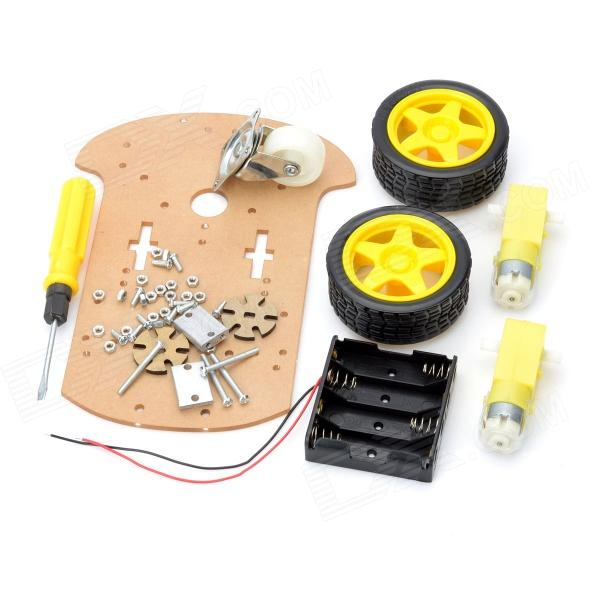
\includegraphics[scale=0.3]{Estrutura.jpg}
             \caption{Estrutura \label{Estrutura}}
         \end{figure}

     \item Ponte H:

        E um circuito que possibilita a um microcontrolador controlar o sentido
        de rotação de um motor, alem de fornecer a corrente necessária para o
        funcionamento deste motor, visto que em geral microcontroladores
        trabalham em corrente e tensão baixas e motores exigem alta potencia.

        Para cada um dos robôs que estão sendo implementados será usada um
        ponte H como a que pode ser vista na figura ~\ref{PonteH} capaz de
        controlar dois motores de corrente continua simultaneamente. 

         \begin{figure}[ht!]
             \centering
             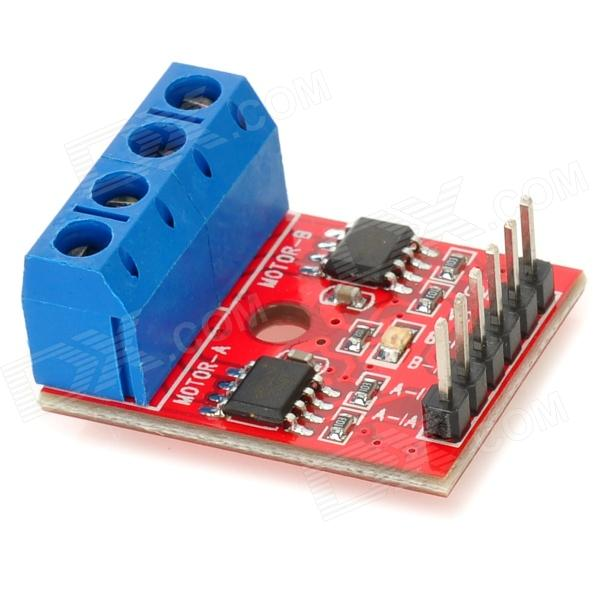
\includegraphics[scale=0.3]{PonteH.jpg}
             \caption{ \label{PonteH}}
         \end{figure}

     \item Giroscópio:  

         Um giroscópio e um instrumento livre para girar em qualquer direção
         mas que quando colocado em rotação tende a se opor a mudanças de
         direção, deste modo utilizando-se de um giroscópio adequado e possível perceber
         qualquer mudança na direção de um objeto.

         Neste trabalho utilizaremos um giroscópio em conjunto com um
         acelerômetro formando um sistemas de navegação inercial. 
     
     \item Acelerômetro:
        
         Como o próprio nome diz acelerômetros são componentes que medem a aceleração, deste
         modo podemos derivar  ,a partir dos dados fornecidos por ele, a distancia percorrida      
         por um objeto em um determinado espaça de tempo.

         Neste projeto usamos um modulo que pode ser visto na figura ~\ref{GiroscopioAcelerometro} que possui um acelerômetro e um
         giroscópio como um sistema de navegação inercial, no qual o giroscópio 
         fornece a direção que o robô esta andando enquanto o acelerômetro a
         distancia que o mesmo já percorreu naquela direção, nos permitindo
         definir a posição atual do robô com base em sua posição inicial.
 

         \begin{figure}[ht!]
             \centering
             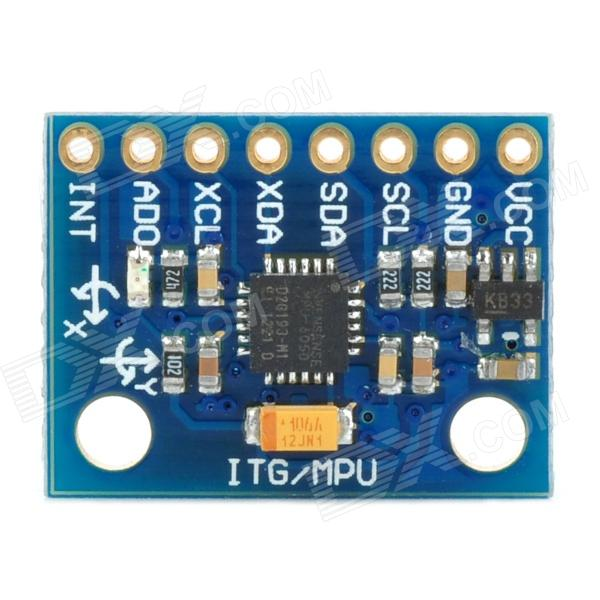
\includegraphics[scale=0.3]{GiroscopioAcelerometro.jpg}
             \caption{ Modulo giroscópio e acelerômetro \label{GiroscopioAcelerometro}}
         \end{figure}

     \item Microcontrolador:  
        
         Um microcontrolador, nada mais é que uma espécie de microprocessador que tem como
        principal finalidade a alta integração. Esses poderosos dispositivos lógicos
        podem integrar elementos, tais como, memória para armazenamento de programas ou
        dados, dispositivos periféricos e interfaces E/S, sendo de um simples pino
        digital a uma interface USB (Universal Serial Bus) ou Ethernet.
        
        O microcontrolador escolhido para esse projeto foi o MSP430G2553,um
        microcontrolador da Texas Instruments com  arquitetura RISC de 16 bits podendo trabalhar a
        uma frequência interna de até 16 MHz, 16kB de memoria Flash, 512B de
        ram e 18 pinos de entrada e saída. 

        Um dos principais motivos para escolha desse microcontrolador e a sua
        facilidade de programação através da plataforma Launchpad, que pode ser
        vista na figura ~\ref{Launchpad} que é uma  plataforma  de prototipagem 
        eletrônica que permite programar e realizar o debug na série
        de microcontroladores MSP430 através da interface USB.

 
         \begin{figure}[ht!]
             \centering
             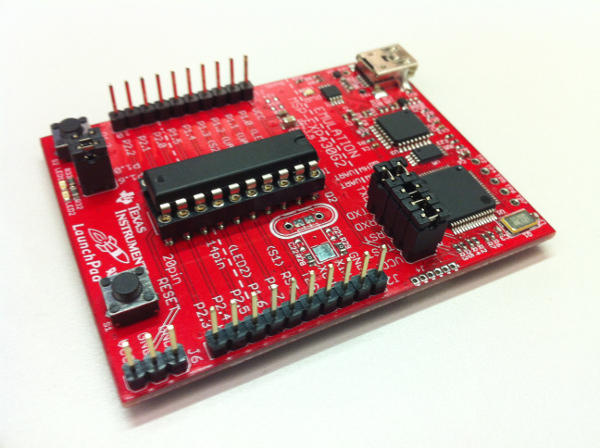
\includegraphics[scale=0.3]{Launchpad.jpg}
             \caption{Launchpad \label{Launchpad}}
         \end{figure}
    
     \item Modulo Wi-Fi:

         Para a comunicação vamos utilizar o módulo RN-XV fabricado pela
         Roving Networks que pode ser visto na imagem ~\ref{WiFi}, é uma solução Wi-Fi
         incorpora o  padrão 802.11 b/g , processador 32 bits, pilha TCP/IP, unidade de gerenciamento de 
         energia e interface para sensor analógico.
         Na configuração mais simples, o hardware requer apenas quatro conexões (PWR, TX, RX e 
         GND) para criar uma conexão de dados sem fio.
         
            \begin{figure}[ht!]
             \centering
             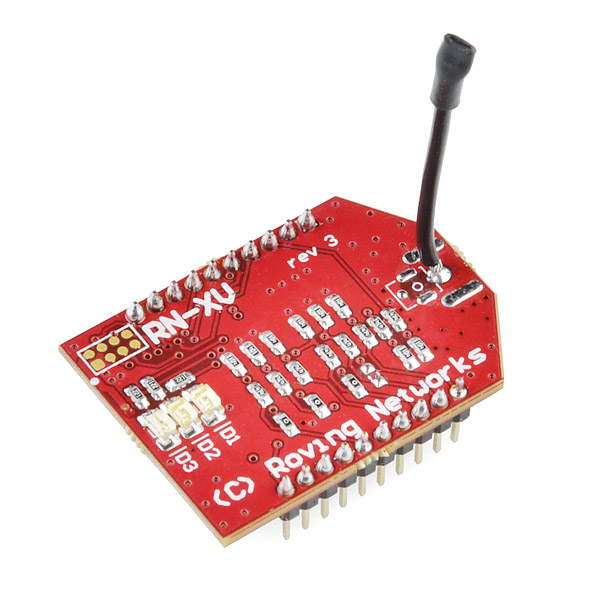
\includegraphics[scale=0.3]{WiFly.jpg}
             \caption{Wi-Fi  \label{WiFi}}
         \end{figure}

\end{itemize}
\section{Módulos}
        O sistema que propomos pode ser modelado como um sistema de tempo real com
        quatro módulos, cada um deles com um conjunto de \textit{tasks} com vários \textit{jobs} cada, são eles,
        locomoção, localização, comunicação e busca, que serão detalhadas a  seguir. 

        \subsection{Locomoção} 
         A partir do trajeto gerado pela busca a locomoção passa a controlar os
         motores de forma a se movimentar na direção correta pela distancia
         necessária. 
         
         O sistema de locomoção dos carros funciona da seguinte
         forma: existem dois motores independentes um acoplado a cada uma das
         rodas da frente a direção e velocidade de cada um deste motores e oque
         define a direção em que o carro vai virar, o carro invariavelmente faz
         uma curva na direção do motor mais veloz.

         Os principais problemas na locomoção são os eventos inesperados, como
         algum obstaculo(geralmente outros carros) ou uma mudança repentina de trajeto por
         parte da busca este tipo de evento requer uma ação imediata deste
         modulo ou pode resultar acidentes e em perda de eficiência.

         As \textit{tasks} previstas para o modulo são citadas abaixo:
         
         \begin{itemize}
            \item Gerar lista de controle: tarefa aperiódica na qual a partir do
                trajeto definido, cria-se uma lista com direções e tempo que deve 
                se manter em cada uma  delas.
            \item Controle dos motores: tarefa periódica que consiste no controle dos motores propriamente
                dito, ou seja passar para a ponte H a velocidade de cada um dos motores
                naquele instante de tempo.

            \item Interrupção: tarefa aperiódica na qual a locomoção disparada
                por um evento inesperado, tarefa na qual o modulo de locomoção
                deve parar imediatamente qualquer umas das outras tarefas que
                esteja fazendo, analisar o evento que a gerou  e mensurar  o
                impacto dele para os \textit{jobs} que ela ainda tem para realizar, em
                muitos casos tendo que reiniciar o processo de locomoção
                chamando novamente o modulo de busca que é responsável por
                definir o trajeto.
         \end{itemize}

        \subsection{Localização} 
        
        A partir de coordenadas geradas por uma constante atualização das
        distâncias percorridas e do posicionamento rotativo, define-se o
        posicionamento relativo dos carros ao ponto inicial.

        O sistema de localização dos carros funciona de acordo com um sistema
        de navegação inercial: é definido um ponto de partida $(x,y)$ e uma
        direção inicial $d$ onde:\\
        $d = { [< : esquerda ||  > : direita || A: cima || V: baixo]}$, 
        para cada carro numa plataforma quadrada de tamanho e um
        conjunto finito de coordenadas pré definidas. A cada movimentação do
        carro, o sistema de localização informa seu ponto atual ao módulo de
        comunicação, essa atualização é baseada em duas informações: 

         \begin{itemize}
             \item Gerada pelo acelerômetro : obtemos a distancia linear
                 percorrido por um carro num determinado espaço de tempo.
             \item Gerado pelo giroscópio : obtemos qualquer mudança de direção
                 de um carro.
         \end{itemize}
        
        A partir dessas duas informações, usamos noções de analises geométricas para
        definirmos a coordenada atual $(x,y)$ por meio de um sistema virtual . 

        Por exemplo, levando em consideração que os carros podem mudar de direção em
        todos os sentidos porém mantendo um variação de
        $45,^{\circ}$ a cada troca de direção:

        Ponto inicial: $(10,10)$ , Direção inicial $(>)$

        Operações:

         \begin{itemize}
            \item acelerômetro: andou 1.
            \item giroscópio: virou a esquerda $(<)$.
            \item acelerômetro: andou 3.
         \end{itemize}
         Ponto atual: $(12,11)$ ,direção atual $(<)$.

         A operação principal do módulo Localização é a atualização constante
         da posição (coordenadas virtuais) do carro, porém há possibilidade de
         haver algumas operações aperiódicas.

         \begin{itemize}
         \item Atualizar coordenadas: Informar localização atualizada periodicamente
         ao módulo comunicação e locomoção, ou seja recalcular o posicionamento dos
         carrinhos de acordo com os dados fornecidos pelo acelerômetro e o
         giroscópio.
         \item Necessidade de atualizar rota: Por questões inesperadas (como
         colisões) o módulo Busca pode ter a necessidade de ajustar uma nova
         rota para evitar tais, para essa operação é imprescindível que o
         módulo Localização envie a posição atual imediata ao módulo Busca. 
         \item Informar Sucesso: Se o posicionamento de um carro corresponder a algum
         ponto da tabela de de Busca fornecida pelo módulo de Comunicação, o
         módulo de Localização envia uma mensagem de “sucesso” para o mesmo,
         delegando a necessidade de atualizar a tabela de pontos desejados.
         \end{itemize}

        \subsection{Comunicação}

        Projetamos e implementamos uma de um protocolo de comunicação que pode
        ser visto na figura ~\ref{protocolo}, existem três \textit{tasks}, duas
        aperiódicas inicializar e informar sucesso, e uma periódica informar
        posição, cada mensagem a ser enviada pelo cliente e representada por
        um retângulo e as mensagens enviadas pelo servidor por uma elipse,
        existem ainda os estados como inicio fim e espera, e um retângulo
        pontilhado que representam clientes externos aos quais o servidor envia
        dados.

         \begin{figure}[ht!]
             \centering
             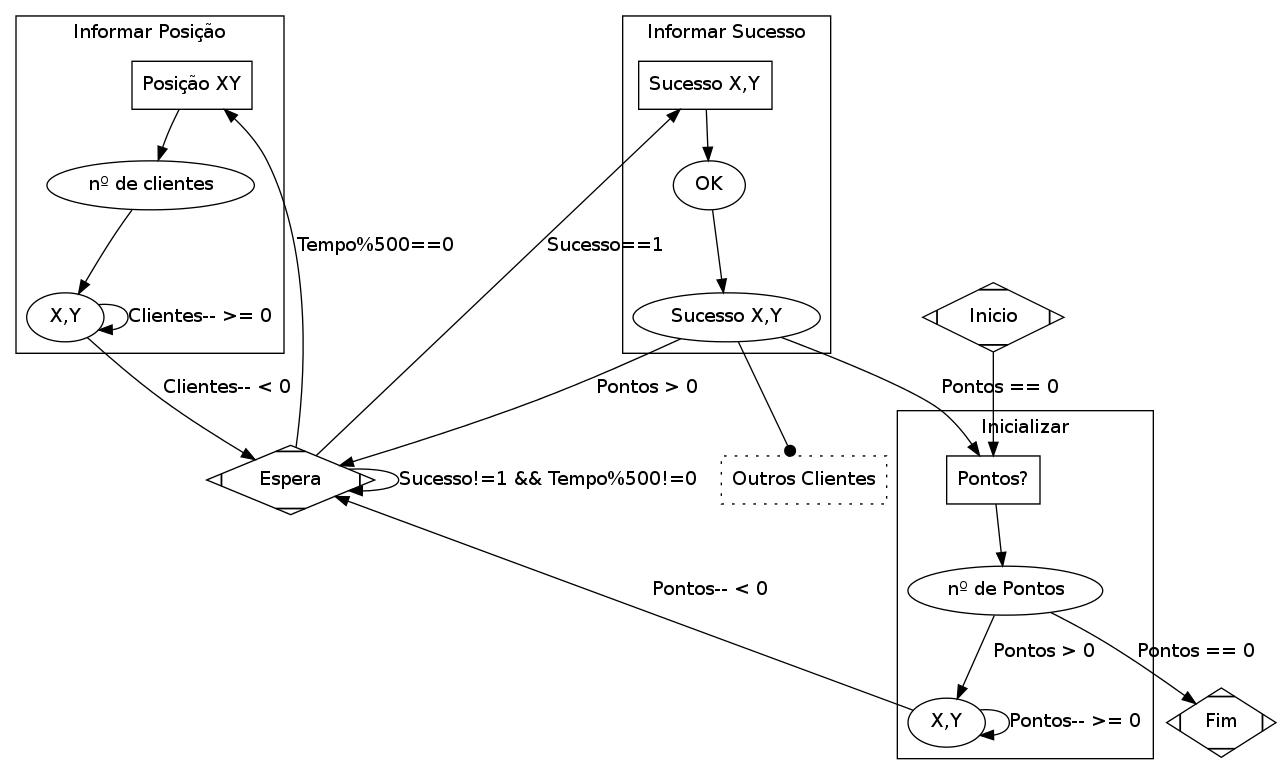
\includegraphics[scale=0.35]{Protocolo.jpg}
             \caption{Protocolo de comunicação \label{protocolo}}
         \end{figure}
       \newpage 
        \subsection{Busca}

        O módulo Busca tem como função definir trajetos aos carros visando
        alcançar todos pontos pre-estabelecidos.

        Para realizar suas tarefas, o módulo Busca recolhe informações para
        indicar onde o carro deve ir, ou seja, o ponto seguinte mais próximo
        almejado. Tais informações são detalhadas a seguir:

        \begin{itemize}
            \item Localização do carro: O módulo Localização envia a coordenada  $(x,y)$  e a
        direção atual do carro ($d = { [< : esquerda ||  > : direita || A: cima || V: baixo]}$) ao módulo Busca.
           \item Pontos almejados: o módulo Comunicação envia para o módulo Busca uma tabela de
        pontos que os carros devem atingir.
        \end{itemize}
        As seguintes informações são peças para a Busca determinar a melhor rota do
        carro ( ponto A) até o ponto mais próximo da tabela de pontos (ponto B). O
        cálculo da melhor rota é baseado em noções de distância entre dois pontos num
        plano. A rota é compreendida por dois segmentos de reta num plano (x,y) , ou
        seja o carro irá percorrer um pedaço do caminho na direção x e outro pedaço na
        direção y, variando a rotatividade do carro. Por exemplo:

        Coordenada do carro: $(3,5)$ , Direção do carro : d =$(>)$\\
        Pontos da tabela: $(9, 15)$, $(1,20)$, $(6,10)$\\
        Ponto mais próximo: $(6,10)$\\
        Rota: ( ande 3; vire para cima, ande 5) $--> ( 3 ,A , 5)$\\

        Coordenada atual do carro : $(6,10)$ , d = $(A)$\\
        Pontos da tabela: $(9,15)$,$(1,20)$\\
        Ponto mais próximo: $( 9,15)$\\
        Rota: $( > , 3 , A , 5 )$\\

        Coordenada atual do carro : $(9,15)$ , d= $(A)$\\
        Pontos da tabela: $(1,20)$\\
        Ponto mais próximo: $( 1,20)$\\
        Rota: $( <,8,V, 5)$

        O principal desafio do módulo Busca são as situações inesperadas, como uma
        colisão ou defeitos de hardware.

        As tasks previstas para o módulo são:
        \begin{itemize}
                \item Calcular rota: De acordo com as informações obtidas pelo módulo
                de Comunicação e Localização, calcula-se a próxima rota de
                busca de um carro por demanda do módulo comunicação, ou seja,
                vai definir rotas até acabar a lista de pontos.
                \item Definir nova rota: Caso haja algum obstáculo no percurso do
                carro ( parede, colisões com outros carros) o módulo de
                Locomoção vai solicitar uma que o processo de Busca para defina
                uma nova rota para o carro.
        \end{itemize}





\section{Escalonamento}
    Como grande parte das \textit{tasks} do projeto são aperiódicas precisamos
    de um modelo de escalonamento que preveja este tipo de \textit{task}, por
    isso optamos por escalonar as tarefas utilizando um servidor periódico, ele
    tem período igual ao maior período aperiódico e seu orçamento e dinâmico
    atualizado pelo escalonador, sendo sempre  o tempo restante ate a execução
    da próxima tarefa periódica.

    Como a maior parte do sistema e extremamente dependente da velocidade dos
    carrinhos o tempo entre as execuções da mesma tarefa periódica e sempre
    muito grande como pode ser visto na tabela ~\ref{tabela}, oque torna o tempo disponível para executar uma determinada
    task muito maior que o período dessa \textit{task}.

\begin{table}
 \caption{ Tabela de tempo de execução e deadlines previstos \label{tabela}}
    \begin{footnotesize}
    \begin{tabular}{|lll|}
    \hline
    Task                                 & Tempo Previsto & Dead Line                                                  \\
    Informar Posição                     & 1 ms           & 500 ms desde a ultima execução                             \\
    Informar sucesso                     & 1 ms           & 100 ms desde de o momento que achou o ponto                \\
    Inicializar                          & 1 ms           & 100 ms desde que o numero de pontos para busca e igual a 0 \\
    Gerar Lista de Controle              & 800 ns         & 100 ms desde o fim da busca                                \\
    Controlar motores                    & 1 ms           & 500 ms desde a ultima execução                             \\
    Evento inesperado                    & 800 ns         & 50 ms desde a detecção                                     \\
     Informar localização a comunicação  & 800 ns         & 100 ms desde o fim da comunicação                          \\
    Informar localização à busca         & 800 ns         & 100 ms desde de a descoberta da localização                \\
    Informar sucesso  a comunicação      & 800 ns         & 100 ms desde de a descoberta da localização                \\
    Calcular rota                        & 1000 ns        & 50 ms desde o que o ultimo ponto foi achado                \\
    Definir nova rota                    & 800 ns         & 50 ms desde o que o um evento inesperado foi detectado     \\ \hline
    \end{tabular}
\end{footnotesize}
\end{table}



\chapter{Resultados Esperados} \label{result}        

Neste trabalho desenvolvemos uma plataforma funcional que
exemplificou um sistema de tempo real engajada na área da computação e
robótica. 

Aprendemos a modelar um sistema de tempo real, entendemos as implicações no que diz
respeito à gerenciar recursos, distribuimos tais recursos às aplicações práticas
como as tarefas propostas(t\textit{tasks} e \textit{jobs}) e fomentamos um discurso sobre a
importância que há na compreensão deste tipo de sistema, são conhecimentos e
experiências bastantes válidos em nossa formação acadêmica.

Além de aprofundar os conhecimentos sobre o tema citado, também tiramos
proveito da experiência prática adquirida na implementação de um sistema
integrado de hardware e software real.

\chapter{Cronograma} \label{cronol}  

\begin{itemize}
     
     \item Modelagem: 15 de agosto a 15 de setembro 
     \item Projeto de Hardware: 16 setembro a 30 de setembro 
     \item Montagem de protótipo e Codificação: 1 outubro a 31 de outubro
     \item Testes e ajustes finais: 1 de novembro a 10 de novembro
     \item Análise de resultados: 11 novembro a 25 de novembro

\end{itemize}

\end{document}
